\documentclass[11pt,ngerman,a4paper]{article}
%Gummi|061|=)
\usepackage{amsmath}
\usepackage{a4wide}
\usepackage{url}
\usepackage{amsthm}
\usepackage{amsbsy}
\usepackage{amssymb}
\usepackage{inputenc}
\usepackage{rotating} 
\usepackage{here}
\usepackage{graphicx}
\usepackage{paralist}
\usepackage{selinput}
\usepackage[separate-uncertainty=true]{siunitx}
\usepackage{booktabs}
\sisetup{}
\SelectInputMappings{%
adieresis={ä},
germandbls={ß},
}
\title{\textbf{Versuch V308: Spulen und Magnetfelder}}
\author{Martin Bieker\\
		Julian Surmann\\
		\\
		Durchgef\"{u}hrt am 20.05.2014\\
		TU Dortmund}
\date{}
\usepackage{graphicx}
\begin{document}
\renewcommand\tablename{Tabelle}
\renewcommand\figurename{Abbildung}
\maketitle
\thispagestyle{empty}
\newpage
\clearpage
\setcounter{page}{1}


\section{Einleitung}
In diesem Versuch soll der Verlauf der magnetischen Feldstärke in verschiedenen Spulenanordnungen gemessen werden. 
\section{Theorie}
Magnetfelder entstehen durch die Bewegung elektrischer Ladungen. Mehr allgemeiner Kram.....

\subsection{Magnetfeld einer langen Spule}
Das Magnetfeld im Innern eine langen Spule kann als homogen angesehen werden. Betrachtet man den Raum ausserhalb der Spule als feldfrei an, so kann die Stärke das magnetischen Feldes näherungsweise mit Hilfe der \textsc{4. Maxwellgleichung} 
\begin{equation}
\oint B\cdot d\vec r = \mu_r\mu_0 I
\end{equation}
berechnet werden. Es ergibt sich:
\
\begin{equation}
B = \mu_r\mu_0\frac{nI}l\mathrm.
\end{equation}
\subsection{Magnetfeld einer Helmholtz-Spule}

\begin{figure}[htp]
\centering
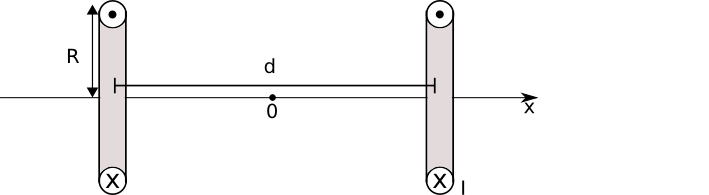
\includegraphics[scale=1.00]{helmholtz.png}
\caption{Schematische Darstellung eines Helmholtz-Spulenpaars}
\label{}
\end{figure}
\begin{equation}
\vec B(x)= \frac{\mu_0I}{2}\left(\frac1{\left(R^2 + (x+\frac d2)^2 \right)^\frac32} + \frac1{\left(R^2 + (x-\frac d2)^2 \right)^\frac32}  \right) \cdot \vec e_x
\end{equation}

\begin{equation}
\frac{d\vec B}{d x} = \frac{-3\mu_0I}{2}\left( \frac{x+\frac d2}{\left(R^2 + (x+\frac d2)^2 \right)^\frac52} + \frac{x-\frac d2}{\left(R^2 + (x-\frac d2)^2 \right)^\frac52}\right) \cdot \vec e_x
\end{equation}
\subsection{Funktionsweise einer Hall-Sonde}
Die in diesem Versuch zu bestimmenden magnetischen Feldstärken, werden mit Hilfe einer Hall-Sonde gemessen. Dieses Messverfahren basiert auf dem \textit{Hall-Effekt}, welcher an dieser Stelle kurz durch Abbildung \ref{hall} erläutert werden soll.  

\begin{figure}[htp]
\centering
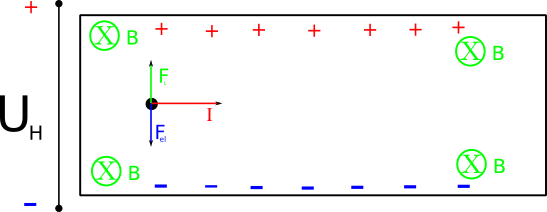
\includegraphics[scale=1.00]{hall.png}
\caption{Schematische Darstellung des Hall-Effekts}
\label{hall}
\end{figure}

An die Hall-sonde wird ein Strom $I$ angelegt. Wird die Sonde von einem magnetischen Feld $\vec B$ durchdrungen, werden die bewegten Ladungen im Inneren durch die Lorentzkraft $F_L$ abgelenkt. Auf Grund dieser Ladungstrennung entsteht ein Elektisches Feld $\vec E$. Dieses wirkt der Ansammlung weiterer Ladungsträger entgegen. Des Weiteren wird durch das Feld eine Spannung erzeugt, die an den Seiten der Sonde abgegriffen werden kann. Im Gleichgewicht gilt:
\[
F_L = F_{el}
\]
Hieraus kann eine Beziehung für das Magnetfeld in Abhängigkeit von der gemessenen Spannung $U_H$ hergeleitet werden:
\[
B = \frac{d}{A_H I } \cdot U_H
\]
Dabei ist $A_H$, genannt Hallkonstante, eine Materialkonstante und $d$ die Dicke der Hall-Sonde. 
Diese Berechnungen werden vom Messgerät, welches in diesem Versuch verwendet wird, intern ausgeführt. Die so gemessene magnetische Feldstärke wird als direkt angezeigt.

\section{Aufbau und Durchführung}
\subsection{Messung an der langen Spule}
Für die Messung an der langen Spule stehen drei Spulenmodule zur Verfügung. Die Spulen sind identisch zueinander und haben folgende Eigenschaften:
\begin{itemize}
\item $n = 3400$
\item $l = \SI{12345678}{\meter}$
\item $d = \SI{0.11}{\meter} \Rightarrow r =  \SI{0.055}{\meter} $.
\end{itemize}
Die Module können hintereinander gesetzt werden, um so längere Spulen zu erzeugen. Die zu vermessende Spule kann an einem Holzlineal auf der x-Achse verschoben werden. Eine longitudinale Hallsonde ist so an einem Stativ befestigt, dass die Sonde auf der Achse der Spule liegt. Durch das Verschieben der Spule wird dann das Magnetfeld im Inneren der Spule an verschiedenen Punkten der Achse gemessen.
\newline
Es werden drei Spulen mit unterschiedlicher Länge untersucht. Dabei wird die Magnetfeldstärke in Abhängigkeit vom Ort x der 
\subsection{Messung an der Helmholtz-Spule}
Die Helmholtz-Spule ist auf einem Sockel befestigt, der an einer Skala das Ablesen der Spulenpositionen ermöglicht. Über den Spulen befindet sich eine Schiene zur Aufnahme der transversalen Hallsonde. An dieser Schiene befindet sich ebenfalls eine Skala. Die Helmholtz-Spule hat folgende Eigenschaften:
\begin{itemize}
\item $n = 100$
\item $l = \SI{0.033}{\meter}$
\item $d = \SI{0.125}{\meter} \Rightarrow r =  \SI{0.0625}{\meter} $.
\end{itemize}

\section{Auswertung}

\section{Quellen}
\begin{enumerate}[{[}1{]}]
\item Entnommen der Praktikumsanleitung \textit{V308: Spulen und Magnetfelder} der TU Dortmund. Download am 26.05.14 unter:\\
 \url{http://129.217.224.2/HOMEPAGE/PHYSIKER/BACHELOR/AP/SKRIPT/Magnetfeld.pdf}
\end{enumerate}

\section{Anhang}
\begin{itemize}
\item Tabellen
\item Auszug aus dem Messheft
\end{itemize}

\begin{table}
\centering
\begin{tabular}{ll}
\toprule
{$x / \si{\centi\meter}$} &{ $B/\si{\milli\tesla}$ }\\
\midrule
1.0 & 2.805\\
2.0 & 2.705\\
3.0 & 2.668\\
4.0 & 2.712\\
5.0 & 2.819\\
11.0 & 2.195\\
12.0 & 1.844\\
13.0 & 1.507\\
14.0 & 1.215\\
15.0 & 0.972\\
16.0 & 0.779\\
17.0 & 0.633\\
18.0 & 0.517\\
19.0 & 0.422\\
20.0 & 0.347\\
\bottomrule
\end{tabular}
\label{}
\caption{}
\end{table}

\begin{table}
\centering
\begin{tabular}{ll}
\toprule
{$x / \si{\centi\meter}$} &{ $B/\si{\milli\tesla}$ }\\
\midrule
1.0 & 3.782\\
1.5 & 3.78\\
7.0 & 2.531\\
8.0 & 2.118\\
9.0 & 1.727\\
10.0 & 1.403\\
11.0 & 1.123\\
12.0 & 0.907\\
13.0 & 0.701\\
14.0 & 0.594\\
15.0 & 0.485\\
16.0 & 0.402\\
17.0 & 0.336\\
18.0 & 0.282\\
19.0 & 0.237\\
\bottomrule
\end{tabular}
\label{}
\caption{}
\end{table}

\begin{table}
\centering
\begin{tabular}{ll}
\toprule
{$x / \si{\centi\meter}$} &{ $B/\si{\milli\tesla}$ }\\
\midrule
1.0 & 2.01\\
2.0 & 1.729\\
3.0 & 1.464\\
4.0 & 1.244\\
5.0 & 1.067\\
6.0 & 0.957\\
7.0 & 0.886\\
8.0 & 0.867\\
9.0 & 0.892\\
10.0 & 0.967\\
11.0 & 1.09\\
12.0 & 1.268\\
13.0 & 1.499\\
14.0 & 1.785\\
15.0 & 2.073\\
\bottomrule
\end{tabular}
\label{}
\caption{}
\end{table}

\begin{table}
\centering
\begin{tabular}{ll}
\toprule
{$x / \si{\centi\meter}$} &{ $B/\si{\milli\tesla}$ }\\
\midrule
10.0 & 7.92\\
11.0 & 7.96\\
12.0 & 7.92\\
13.0 & 7.93\\
14.0 & 8.01\\
15.0 & 8.17\\
16.0 & 8.39\\
17.0 & 8.54\\
18.0 & 8.63\\
19.0 & 8.61\\
20.0 & 8.5\\
21.0 & 8.33\\
22.0 & 8.15\\
23.0 & 7.99\\
24.0 & 7.9\\
25.0 & 7.91\\
26.0 & 7.94\\
27.0 & 7.92\\
28.0 & 7.79\\
29.0 & 7.5\\
30.0 & 7.03\\
31.0 & 6.49\\
32.0 & 5.7\\
33.0 & 4.8\\
34.0 & 3.96\\
35.0 & 3.2\\
36.0 & 2.51\\
37.0 & 1.98\\
38.0 & 1.59\\
39.0 & 1.27\\
40.0 & 1.04\\
41.0 & 0.86\\
\bottomrule
\end{tabular}
\label{}
\caption{}
\end{table}

\begin{table}
\centering
\begin{tabular}{ll}
\toprule
{$x / \si{\centi\meter}$} &{ $B/\si{\milli\tesla}$ }\\
\midrule
10.0 & 2.71\\
11.0 & 3.49\\
12.0 & 4.53\\
13.0 & 5.78\\
14.0 & 6.89\\
15.0 & 8.2\\
16.0 & 9.4\\
17.0 & 10.31\\
18.0 & 11.0\\
19.0 & 11.36\\
20.0 & 11.5\\
21.0 & 11.46\\
22.0 & 11.33\\
23.0 & 11.22\\
24.0 & 11.2\\
25.0 & 11.28\\
26.0 & 11.39\\
27.0 & 11.41\\
28.0 & 11.26\\
29.0 & 10.88\\
30.0 & 10.19\\
31.0 & 9.34\\
32.0 & 8.24\\
33.0 & 7.14\\
34.0 & 5.7\\
35.0 & 4.6\\
36.0 & 3.63\\
37.0 & 2.83\\
38.0 & 2.2\\
39.0 & 1.77\\
40.0 & 1.41\\
41.0 & 1.14\\
42.0 & 0.96\\
43.0 & 0.81\\
44.0 & 0.68\\
45.0 & 0.58\\
46.0 & 0.51\\
47.0 & 0.45\\
48.0 & 0.4\\
49.0 & 0.35\\
50.0 & 0.32\\
\bottomrule
\end{tabular}
\label{}
\caption{}
\end{table}

\begin{table}
\centering
\begin{tabular}{ll}
\toprule
{$x / \si{\centi\meter}$} &{ $B/\si{\milli\tesla}$ }\\
\midrule
10.0 & 0.35\\
11.0 & 0.42\\
12.0 & 0.47\\
13.0 & 0.55\\
14.0 & 0.66\\
15.0 & 0.81\\
16.0 & 0.97\\
17.0 & 1.19\\
18.0 & 1.5\\
19.0 & 1.9\\
20.0 & 2.45\\
21.0 & 3.09\\
22.0 & 4.09\\
23.0 & 5.15\\
24.0 & 6.45\\
25.0 & 7.61\\
26.0 & 8.66\\
27.0 & 9.35\\
28.0 & 9.8\\
29.0 & 9.86\\
30.0 & 9.49\\
31.0 & 8.83\\
32.0 & 7.93\\
33.0 & 6.79\\
34.0 & 5.58\\
35.0 & 4.31\\
36.0 & 3.43\\
37.0 & 2.71\\
38.0 & 2.08\\
39.0 & 1.62\\
40.0 & 1.29\\
41.0 & 1.05\\
42.0 & 0.87\\
43.0 & 0.72\\
44.0 & 0.6\\
45.0 & 0.52\\
46.0 & 0.44\\
47.0 & 0.38\\
48.0 & 0.34\\
49.0 & 0.28\\
50.0 & 0.26\\
\bottomrule
\end{tabular}
\label{}
\caption{}
\end{table}


\end{document}
